\section{View}
The UI will be looking like: \\
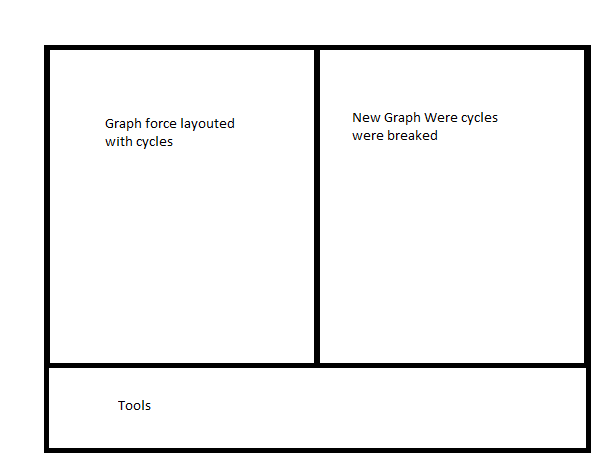
\includegraphics[scale=0.5]{parts/UIToolbarBottom}
or 
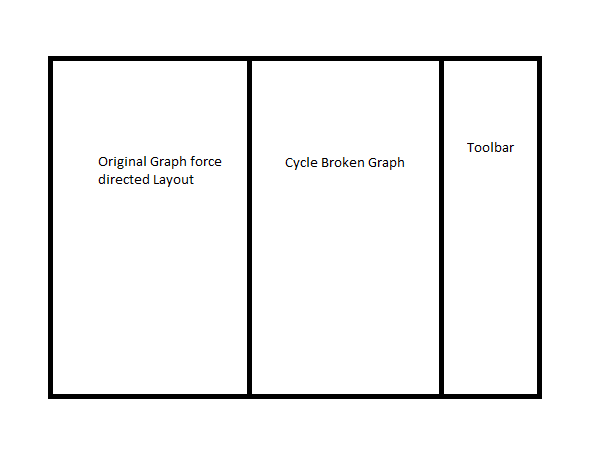
\includegraphics[scale=0.5]{parts/UIToolbarRight}\\
\begin{list}{-}{}
\item The left Graph will bew showing the original graph (concernig edges).
\item The right graph will have it's nodes at the same place as the left graph.
\item Nodes will be a default size
\item Nodes in both graphs will be coloured dynamically
\begin{list}{-}{}
\item Currently (both) used node will be coloured green
\item Sources (left graph) will be colured (yellow maybe?)
\item Sinks (left graph) will be colured (red maybe?)
\end{list}
\item Edges of the current active Node may be coloured (right graph) (in vs. out-degree)
\begin{list}{-}{}
\item Incoming edges are coloured (blue?)
\item Outgoing edges are coloures (purple?)
\end{list}
\end{list}




